\section{Pattern classification on Non-linearly Separable Data}
\subsection{Non-Linear SVM with One-Against-The-Rest Approach}


The given synthetic data is classified using Support Vector Classifier with One Vs the Rest Approach. Sklearn was used to implement the method. It was tried with polynomial and gaussian kernels. Let us look at the performance of the various models by changing different parameters. 

Both the models can handle the data very well and the best model in both the cases gave a 100$\%$  test accuracy. In case of gaussian kernels, gamma as 10 gave the best model where gamma is the width parameter. In the case of polynomial kernels, setting degree as 4, coeff as 1 and gamma as 10 gave the best model.  In both the cases, the validation accuracy was also 100$\%$.


% -----------------------------------------------------------
{\rowcolors{3}{green!40!yellow!10}{green!0!yellow!30}
\begin{table}[!h]
\centering
\begin{tabular}{ |c|c|c|  }
\hline
\rowcolor{lightgray} Model & Training Accuracy & Val Accuracy\\
\hline
C=1 & 98.34$\%$  & 100$\%$  \\ 
\hline
C=0.5 & 97.84$\%$  & 100$\%$  \\ 
\hline
C=2 & 99.17$\%$  & 100$\%$  \\ 
\hline
C=4 & 99.5$\%$  & 100$\%$  \\ 
\hline
gamma=0.1 & 52.17$\%$  & 68.89$\%$  \\ 
\hline
gamma=1 & 90.5$\%$  & 91.12$\%$  \\ 
\hline
gamma=10 & 99.67$\%$  & 100$\%$  \\ 
\hline
\end{tabular}
\caption{Performance of various SVM Models with gaussian kernels}.
\label{table:1}
\end{table}
}

\newpage
% -----------------------------------------------------------
{\rowcolors{3}{green!40!yellow!10}{green!0!yellow!30}
\begin{table}[!h]
\centering
\begin{tabular}{ |c|c|c|  }
\hline
\rowcolor{lightgray} Model & Training Accuracy & Val Accuracy\\
\hline
Deg=2 / coeff=0 & 36.17$\%$  & 31.12$\%$  \\ 
\hline
Deg=2 / coeff=1 & 63.0$\%$  & 73.34$\%$  \\ 
\hline
Deg=2 / coeff=1 / gamma=1 & 57.49$\%$  & 68.89$\%$  \\ 
\hline
Deg=2 / coeff=1 / gamma=10 & 64.5$\%$  & 75.56$\%$  \\ 
\hline
Deg=3 / coeff=1 / gamma=10 & 99.17$\%$  & 100$\%$  \\ 
\hline
Deg=4 / coeff=1 / gamma=10 & 99.67$\%$  & 100$\%$  \\ 
\hline
\end{tabular}
\caption{Performance of various SVM Models with polynomials kernels}.
\label{table:3}
\end{table}
}

\subsubsection{Plots for Gaussian Kernel SVM}

%---------------------------------------------------------

\begin{figure}[!ht]
    \centering
    \begin{subfigure}[t]{0.5\textwidth}
        \centering
        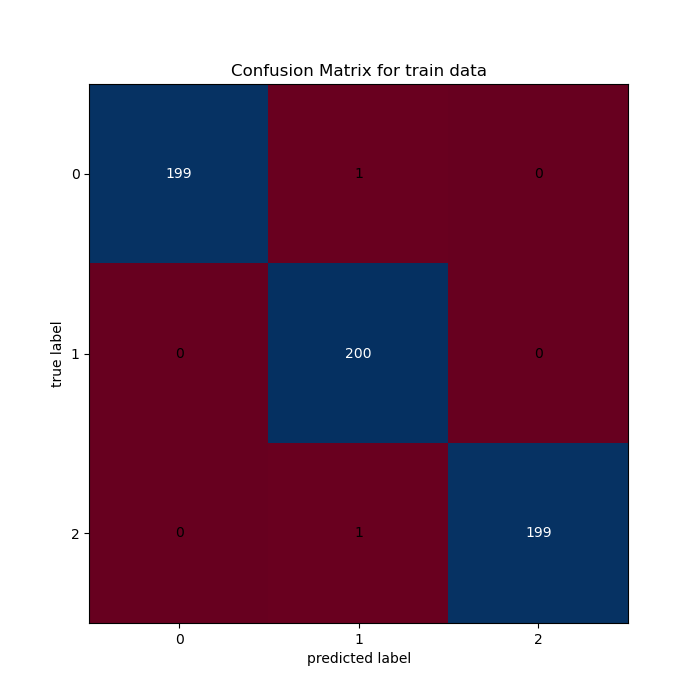
\includegraphics[height=2.5in]{Dataset_1b/SVM/SVC_Gaussian_cmatrix_train_data.png}
        \caption{Confusion Matrix for training data}
    \end{subfigure}%
    ~ 
    \begin{subfigure}[t]{0.5\textwidth}
        \centering
        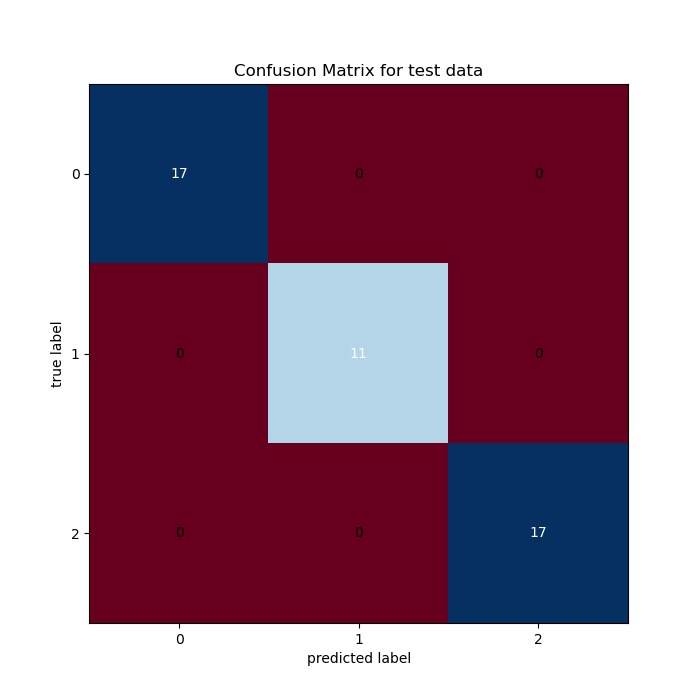
\includegraphics[height=2.5in]{Dataset_1b/SVM/SVC_Gaussian_cmatrix_test_data.png}
        \caption{Confusion Matrix for test data}
    \end{subfigure}%
    ~
    \caption{Confusion Matrix for the best model}
    \label{fig:13}
\end{figure}

%----------------------------------------------------------
\begin{figure}[!ht]
    \centering
    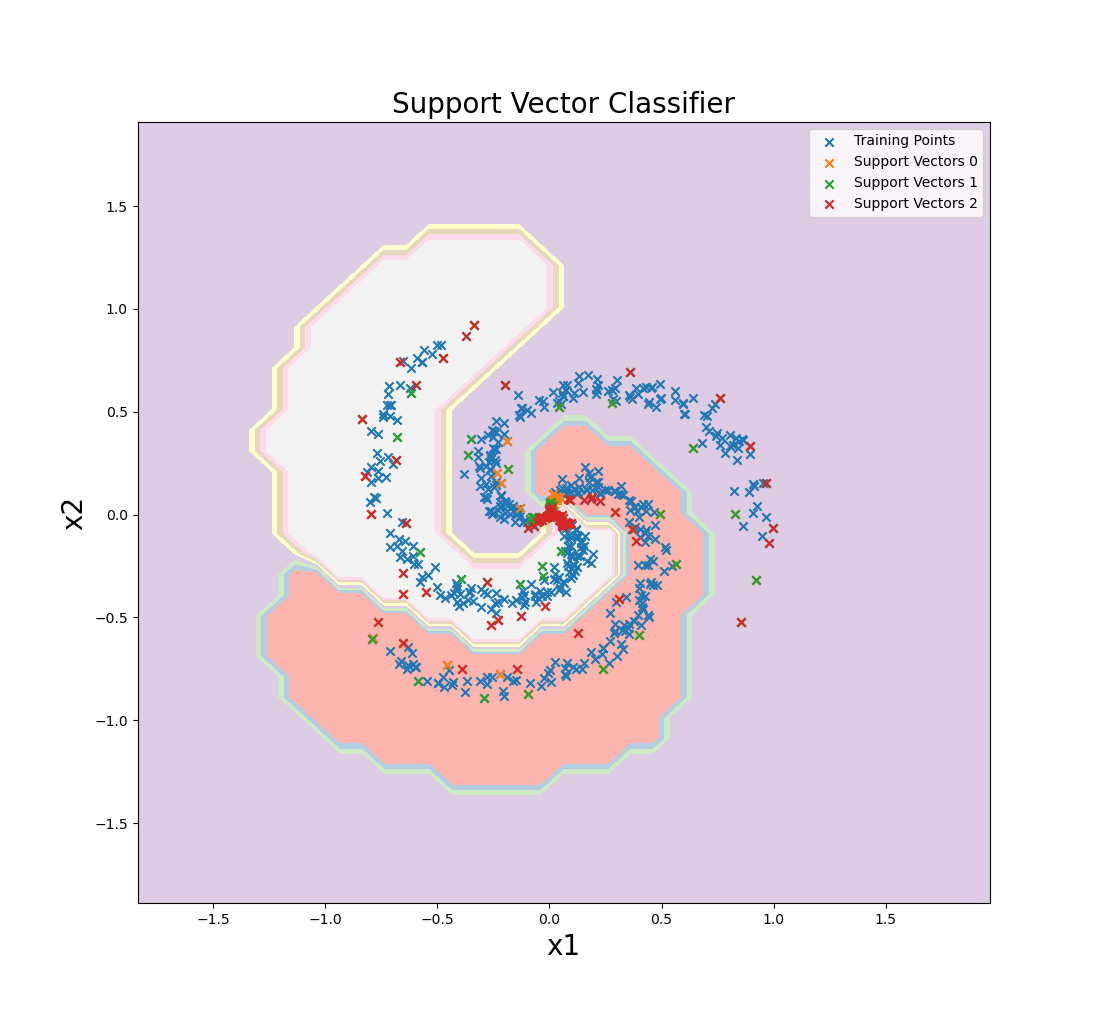
\includegraphics[height=3.5in]{Dataset_1b/SVM/SVC_Gaussian.png}
    \caption{Decision plot for the best model}
    \label{fig:14}
\end{figure}



\begin{figure}[!ht]
    \centering
    \begin{subfigure}[t]{0.3\textwidth}
        \centering
        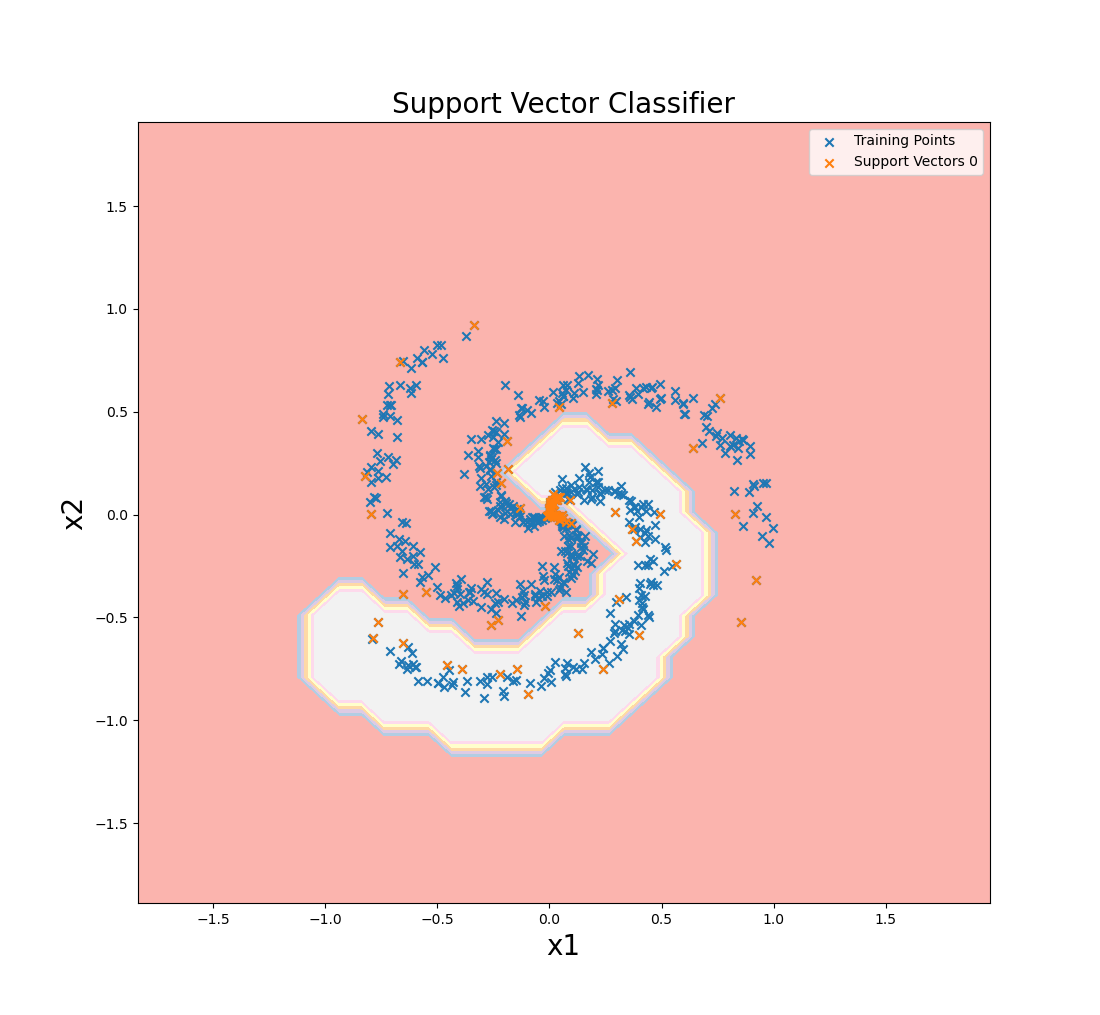
\includegraphics[height=1.75in]{Dataset_1b/SVM/test1.png}
    \end{subfigure}%
    ~ 
    \begin{subfigure}[t]{0.3\textwidth}
        \centering
        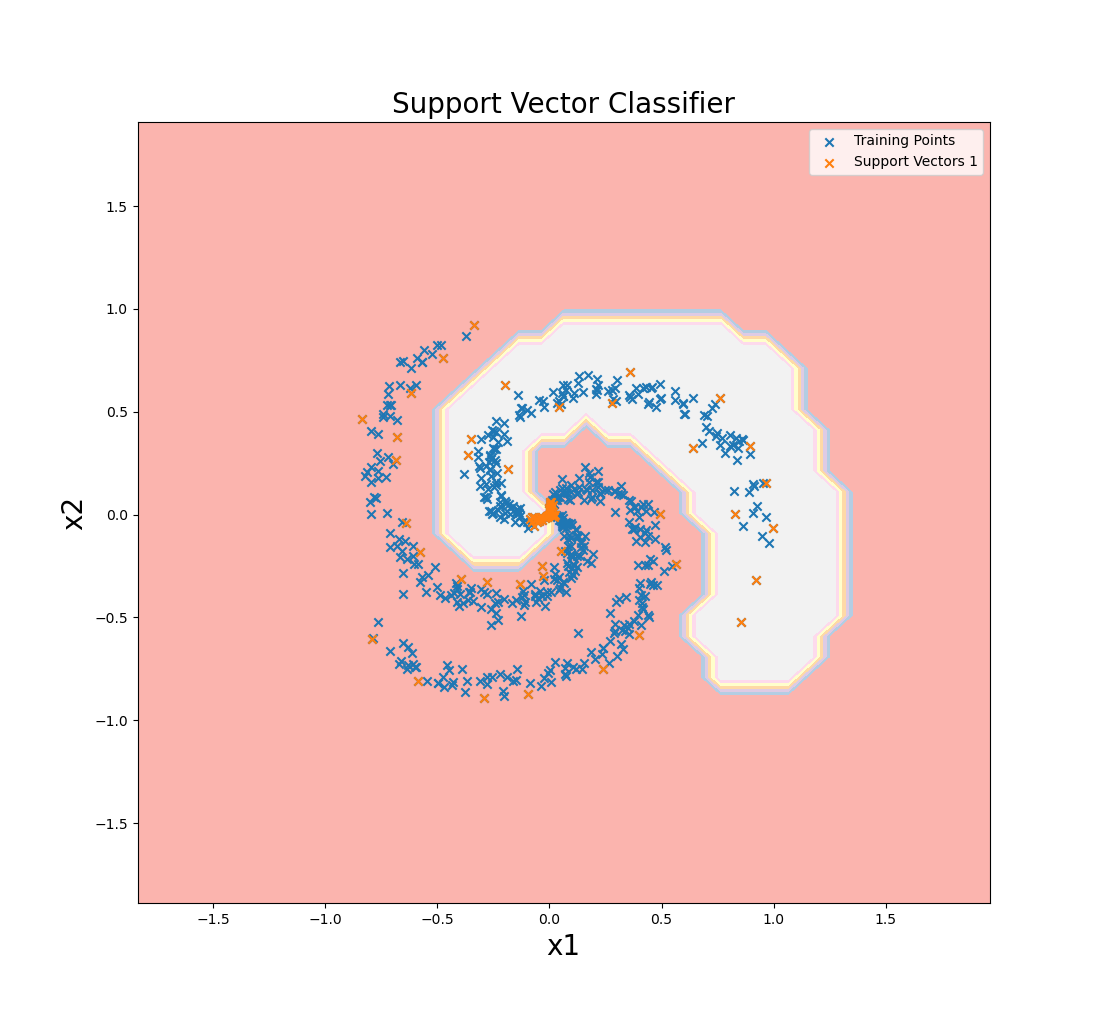
\includegraphics[height=1.75in]{Dataset_1b/SVM/test2.png}
    \end{subfigure}%
    ~
    \begin{subfigure}[t]{0.3\textwidth}
        \centering
        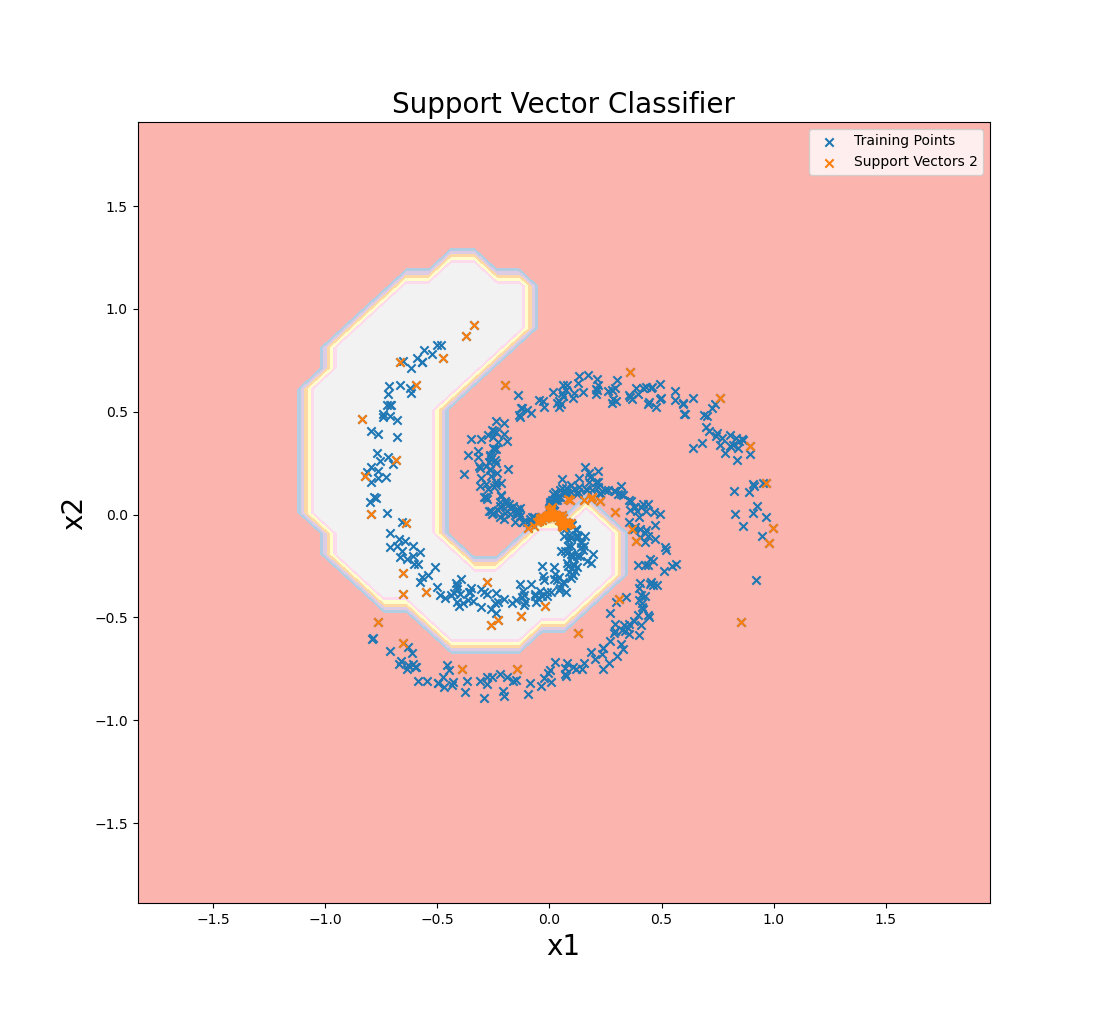
\includegraphics[height=1.75in]{Dataset_1b/SVM/test3.png}
    \end{subfigure}%
    \caption{Various Decision Plots for 3 classifiers used in One Vs Rest Approach}
    \label{fig:13}
\end{figure}



\newpage
\subsubsection{Plots for Polynomial Kernel SVM}

%---------------------------------------------------------

\begin{figure}[!ht]
    \centering
    \begin{subfigure}[t]{0.5\textwidth}
        \centering
        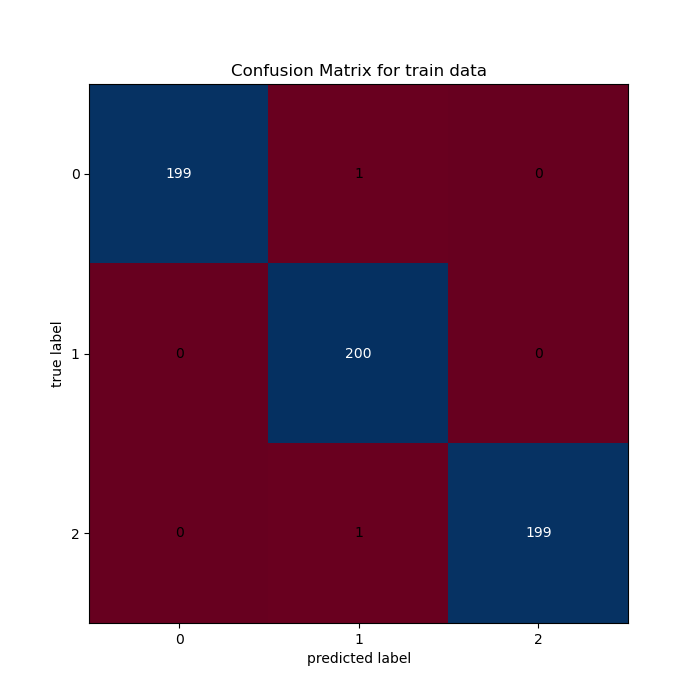
\includegraphics[height=2.5in]{Dataset_1b/SVM/SVC_poly_cmatrix_train_data.png}
        \caption{Confusion Matrix for training data}
    \end{subfigure}%
    ~ 
    \begin{subfigure}[t]{0.5\textwidth}
        \centering
        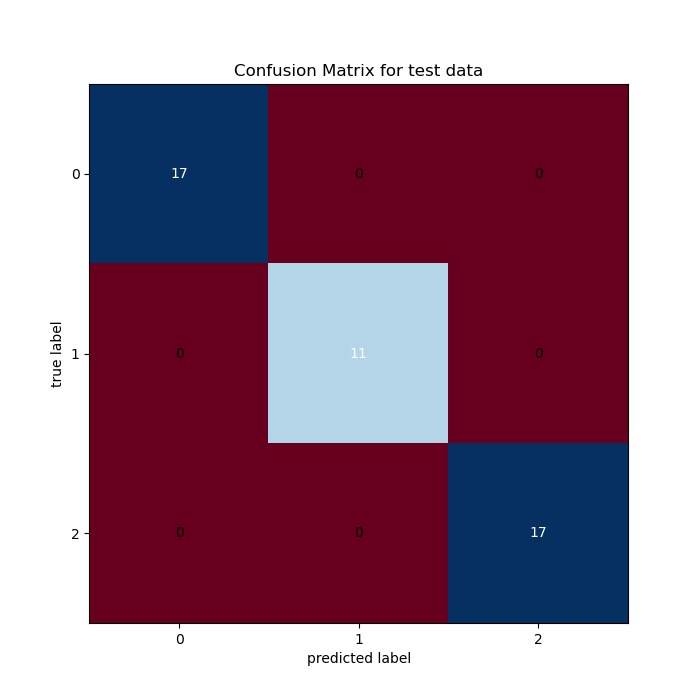
\includegraphics[height=2.5in]{Dataset_1b/SVM/SVC_poly_cmatrix_test_data.png}
        \caption{Confusion Matrix for test data}
    \end{subfigure}%
    ~
    \caption{Confusion Matrix for the best model}
    \label{fig:13}
\end{figure}

%----------------------------------------------------------
\begin{figure}[!ht]
    \centering
    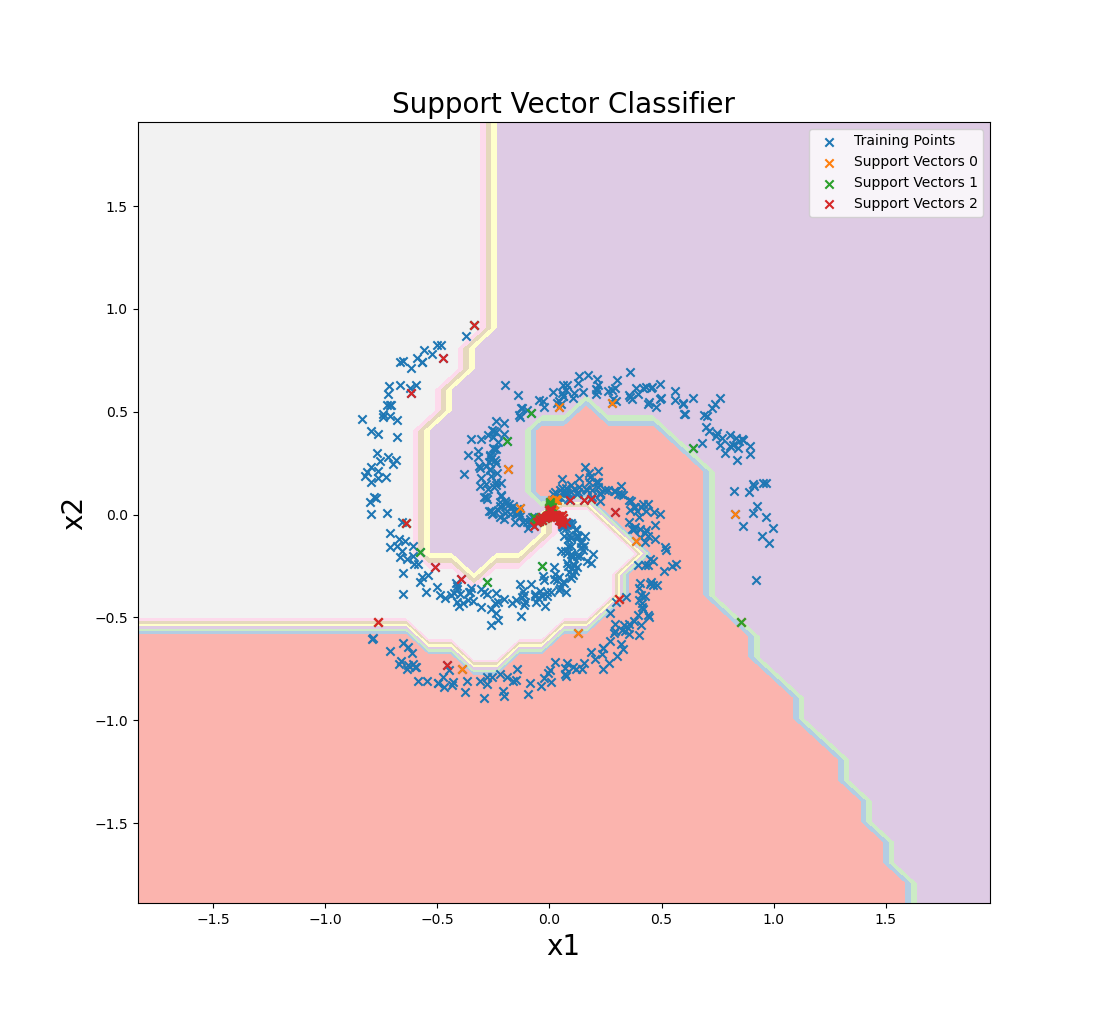
\includegraphics[height=3.5in]{Dataset_1b/SVM/SVC_Poly.png}
    \caption{Decision plot for the best model}
    \label{fig:14}
\end{figure}

\begin{figure}[!ht]
    \centering
    \begin{subfigure}[t]{0.33\textwidth}
        \centering
        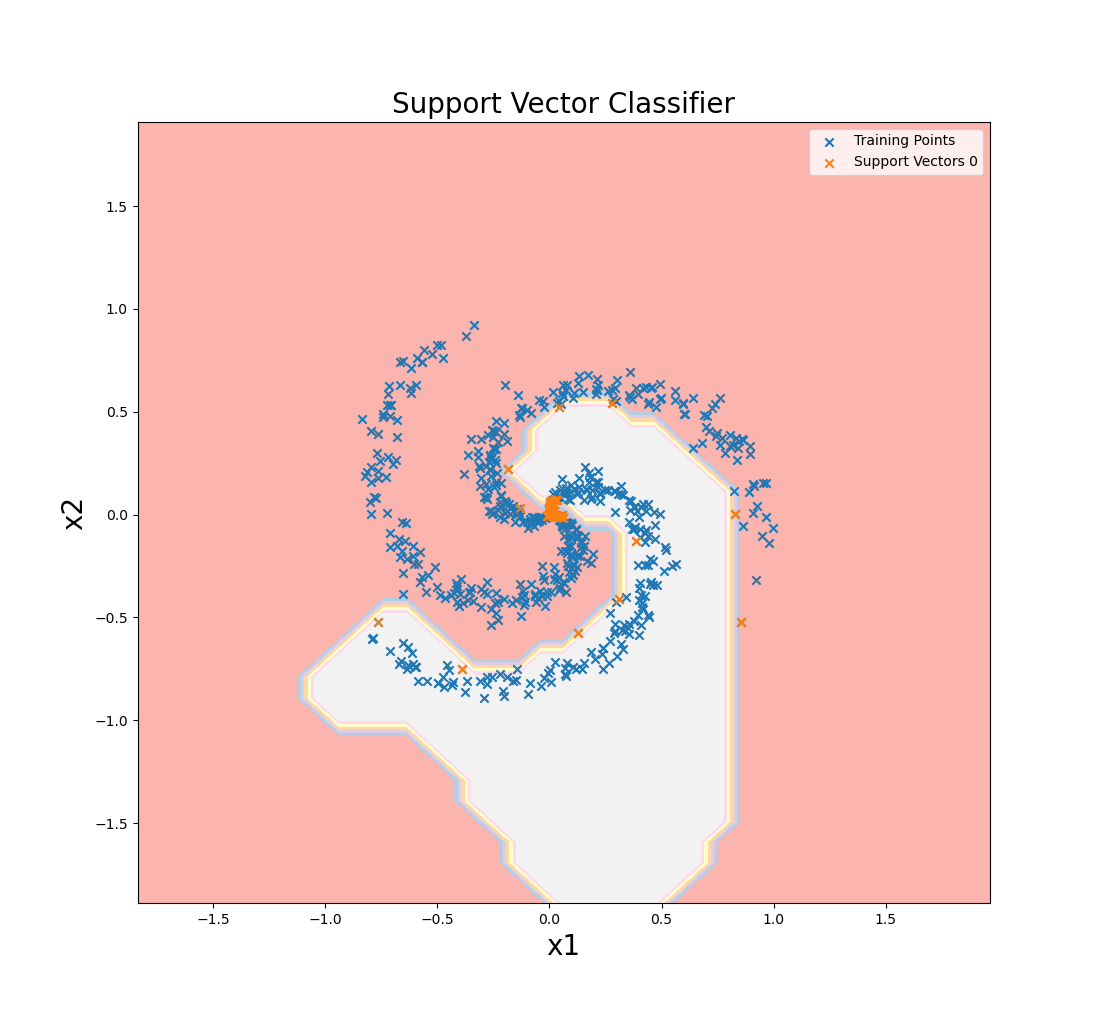
\includegraphics[height=1.75in]{Dataset_1b/SVM/test4.png}
    \end{subfigure}%
    ~ 
    \begin{subfigure}[t]{0.33\textwidth}
        \centering
        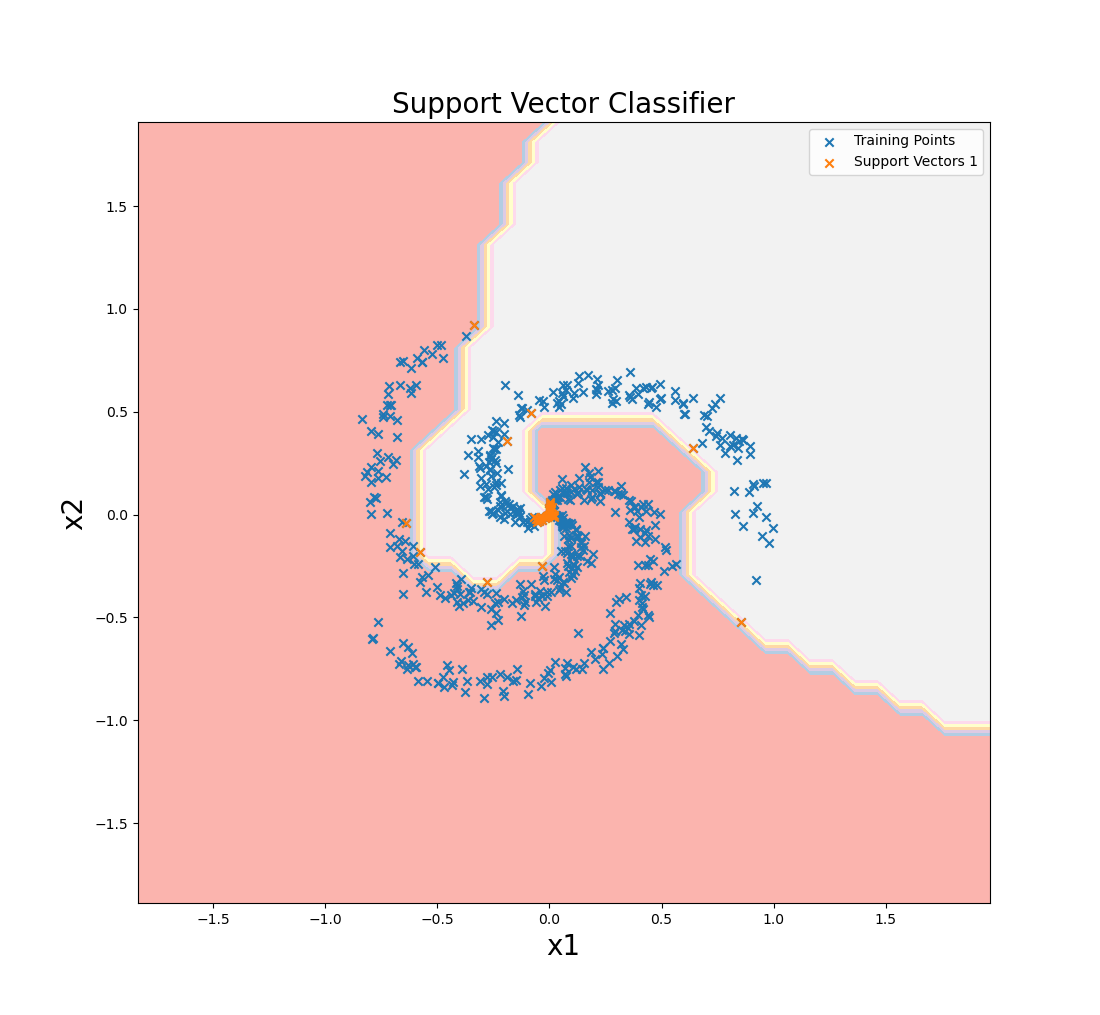
\includegraphics[height=1.75in]{Dataset_1b/SVM/test5.png}
    \end{subfigure}%
    ~
    \begin{subfigure}[t]{0.33\textwidth}
        \centering
        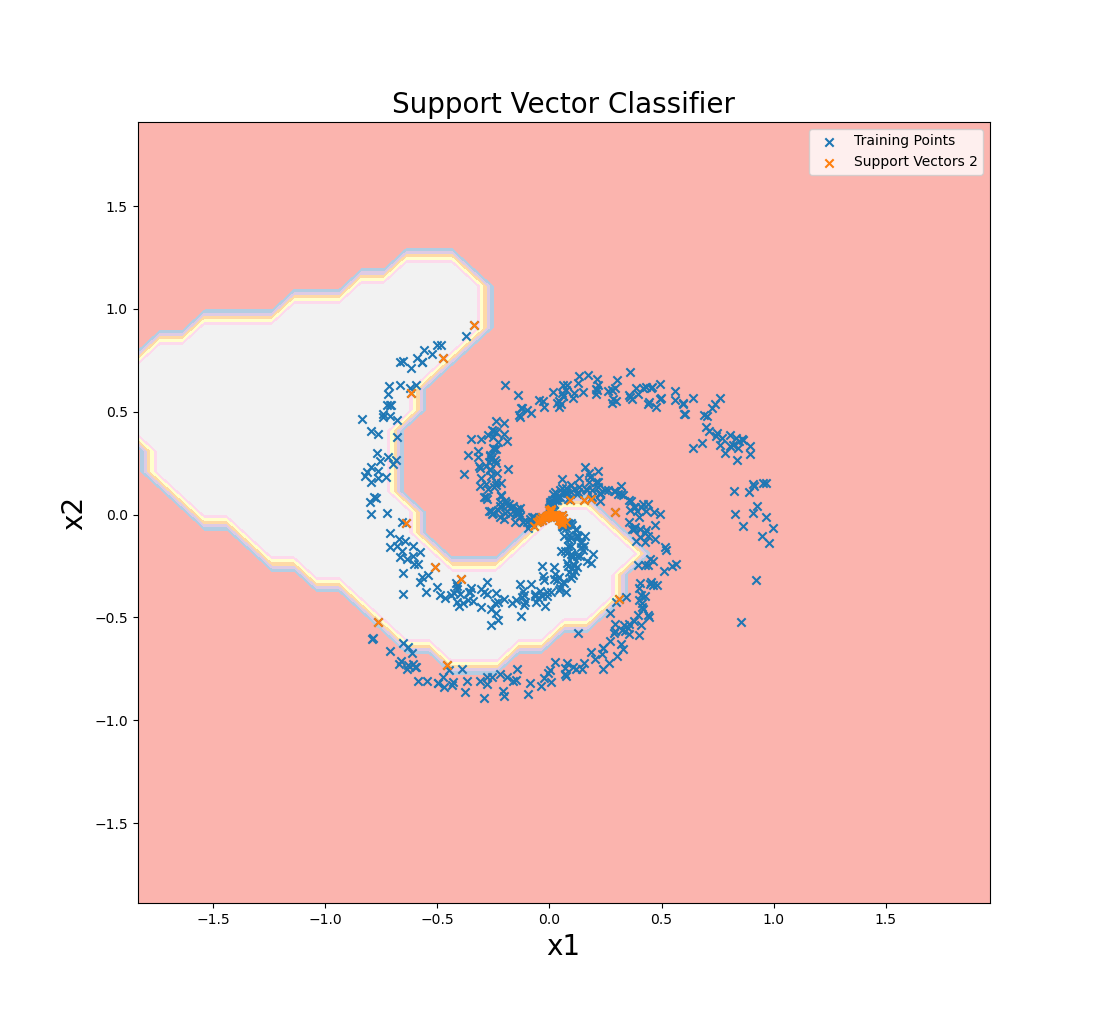
\includegraphics[height=1.75in]{Dataset_1b/SVM/test6.png}
    \end{subfigure}%
    \caption{Various Decision Plots for 3 classifiers used in One V sRestApproach}
    \label{fig:13}
\end{figure}

\newpage
\section{Static Pattern classification on Real World Data}

\subsection{SVM with Gaussian Kernel}
The given real world data is classified using Support Vector Classifier with One Vs the Rest Approach. Sklearn was used to implement the method. It was tried with gaussian kernels. Let us look at the performance of the various models by changing different parameters. The best model was observed for gamma=20 which is the width parameter and the test accuracy was 56.14$\%$.



% -----------------------------------------------------------
{\rowcolors{3}{green!40!yellow!10}{green!0!yellow!30}
\begin{table}[!h]
\centering
\begin{tabular}{ |c|c|c|  }
\hline
\rowcolor{lightgray} Model & Training Accuracy & Val Accuracy\\
\hline
C=1 & 78.24$\%$  & 55$\%$  \\ 
\hline
C=3 & 85.47$\%$  & 57.78$\%$  \\ 
\hline
C=6 & 90.01$\%$  & 57.22$\%$  \\ 
\hline
C=10 & 93.26$\%$  & 53.33$\%$  \\ 
\hline
C=15 & 95.29$\%$  & 56.11$\%$  \\ 
\hline
gamma=1 & 67.53$\%$  & 51.92$\%$  \\ 
\hline
gamma=10 & 93.83$\%$  & 58.46$\%$  \\ 
\hline
gamma=20 & 98.86$\%$  & 62.84$\%$  \\ 
\hline
\end{tabular}
\caption{Performance of various SVM Models with gaussian kernels}.
\label{table:3}
\end{table}
}

%---------------------------------------------------------

\begin{figure}[!ht]
    \centering
    \begin{subfigure}[t]{0.5\textwidth}
        \centering
        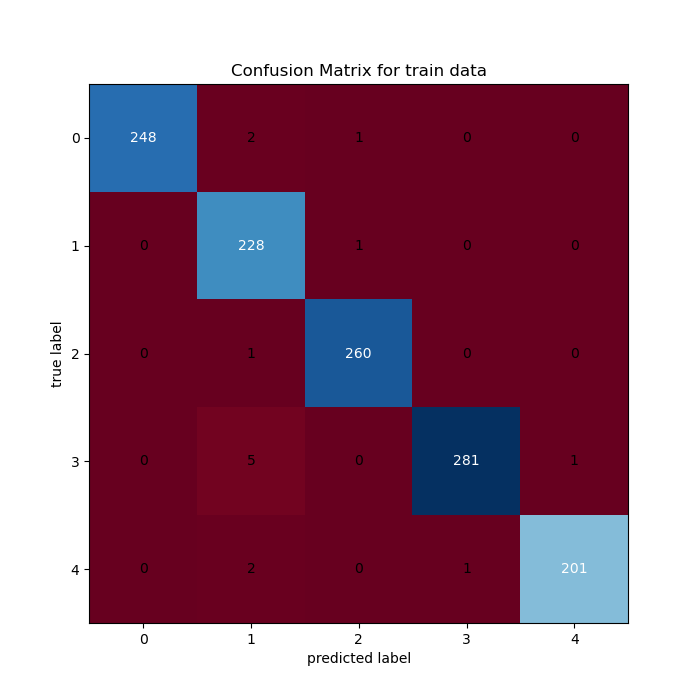
\includegraphics[height=2.5in]{Dataset_2a/dataset_2a_cmatrix_train_data_svc.png}
        \caption{Confusion Matrix for training data}
    \end{subfigure}%
    ~ 
    \begin{subfigure}[t]{0.5\textwidth}
        \centering
        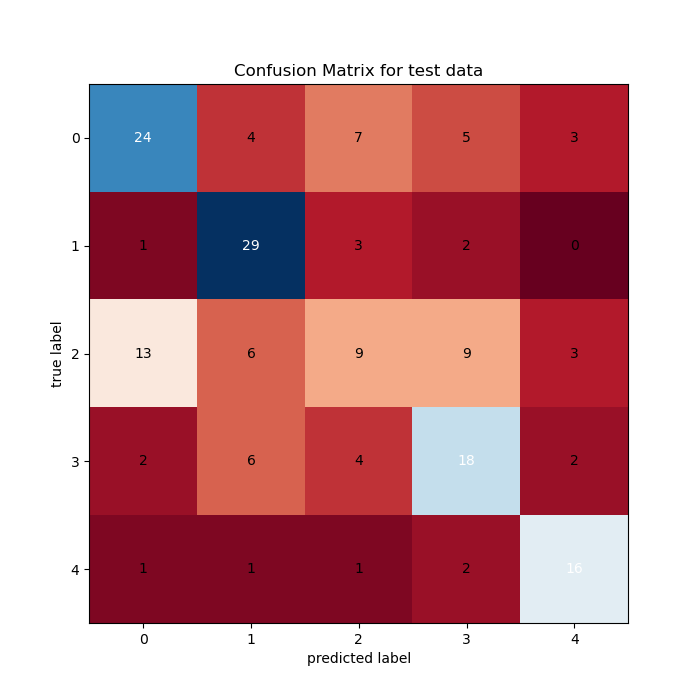
\includegraphics[height=2.5in]{Dataset_2a/dataset_2a_cmatrix_test_data_svc.png}
        \caption{Confusion Matrix for test data}
    \end{subfigure}%
    ~
    \caption{Confusion Matrix for the best model}
    \label{fig:13}
\end{figure}

%---------------------------------------------------------